% 120-20(120쪽) — 두 사차함수 y=f(x), y=g(x) 의 그래프가 x=-7, -4, 0, 5 에서 만나 생기는 세 도형 A, B, C. 스캔 화질이 낮아 TikZ 로 다시 그림.
% 라벨은 원문 그대로 y·x·O·-7·-4·5·A·B·C·y=f(x)·y=g(x) 와 원문의 점선 세 개만. 세 넓이(4, 6, 11)는 그림에서 잴 수 없게 개략 모양으로 그렸다.
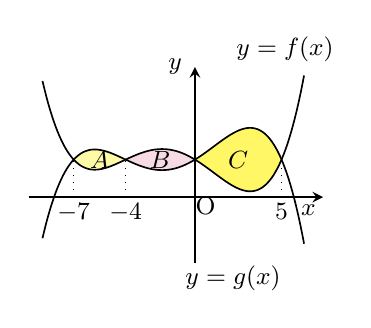
\begin{tikzpicture}[xscale=0.22, yscale=0.28, line width=0.5pt]
  \fill[yellow!35] plot[domain=-7:-4, samples=40] (\x, {1.7+0.0034*(\x+7)*(\x+4)*\x*(\x-5)}) -- plot[domain=-4:-7, samples=40] (\x, {1.7-0.0034*(\x+7)*(\x+4)*\x*(\x-5)}) -- cycle;
  \fill[purple!14] plot[domain=-4:0, samples=50] (\x, {1.7+0.0034*(\x+7)*(\x+4)*\x*(\x-5)}) -- plot[domain=0:-4, samples=50] (\x, {1.7-0.0034*(\x+7)*(\x+4)*\x*(\x-5)}) -- cycle;
  \fill[yellow!60] plot[domain=0:5, samples=60] (\x, {1.7+0.0034*(\x+7)*(\x+4)*\x*(\x-5)}) -- plot[domain=5:0, samples=60] (\x, {1.7-0.0034*(\x+7)*(\x+4)*\x*(\x-5)}) -- cycle;
  \draw[->, >=stealth, line width=0.7pt] (-9.6,0) -- (7.4,0) node[below left=-1pt, font=\small] {$x$};
  \draw[->, >=stealth, line width=0.7pt] (0,-3.0) -- (0,5.9) node[left=1pt, font=\small] {$y$};
  \draw[line width=0.6pt, domain=-8.8:6.3, samples=140] plot (\x, {1.7+0.0034*(\x+7)*(\x+4)*\x*(\x-5)});
  \draw[line width=0.6pt, domain=-8.8:6.3, samples=140] plot (\x, {1.7-0.0034*(\x+7)*(\x+4)*\x*(\x-5)});
  \draw[dotted, line width=0.5pt] (-7,0) -- (-7,1.7);
  \draw[dotted, line width=0.5pt] (-4,0) -- (-4,1.7);
  \draw[dotted, line width=0.5pt] (5,0) -- (5,1.7);
  \node[below right=-1pt, font=\small, inner sep=1pt] at (0,0) {$\mathrm{O}$};
  \node[below, font=\small, inner sep=2pt] at (-7,0) {$-7$};
  \node[below, font=\small, inner sep=2pt] at (-4,0) {$-4$};
  \node[below, font=\small, inner sep=2pt] at (5,0) {$5$};
  \node[font=\small] at (-5.5,1.7) {$A$};
  \node[font=\small] at (-2,1.7) {$B$};
  \node[font=\small] at (2.5,1.7) {$C$};
  \node[font=\small] at (5.2,6.7) {$y=f(x)$};
  \node[font=\small] at (2.2,-3.7) {$y=g(x)$};
\end{tikzpicture}
